\documentclass[border=14pt]{standalone}

\usepackage{amsmath}
\usepackage{amssymb}
\usepackage{xcolor}
\usepackage{tikz}
\usetikzlibrary{arrows.meta,positioning,fit,backgrounds,calc,shapes.geometric,decorations.pathreplacing,decorations.markings}

\definecolor{shellink}{RGB}{31,58,95}
\definecolor{attnfill}{RGB}{224,236,247}
\definecolor{attnline}{RGB}{54,104,158}
\definecolor{ffnfill}{RGB}{233,242,229}
\definecolor{ffnline}{RGB}{85,132,68}
\definecolor{normfill}{RGB}{247,240,226}
\definecolor{normline}{RGB}{160,124,54}
\definecolor{detailfill}{RGB}{245,245,248}
\definecolor{residual}{RGB}{176,66,52}
\definecolor{shapetext}{RGB}{92,92,102}

\newcommand{\shape}[1]{\textcolor{shapetext}{\scriptsize$#1$}}

\begin{document}
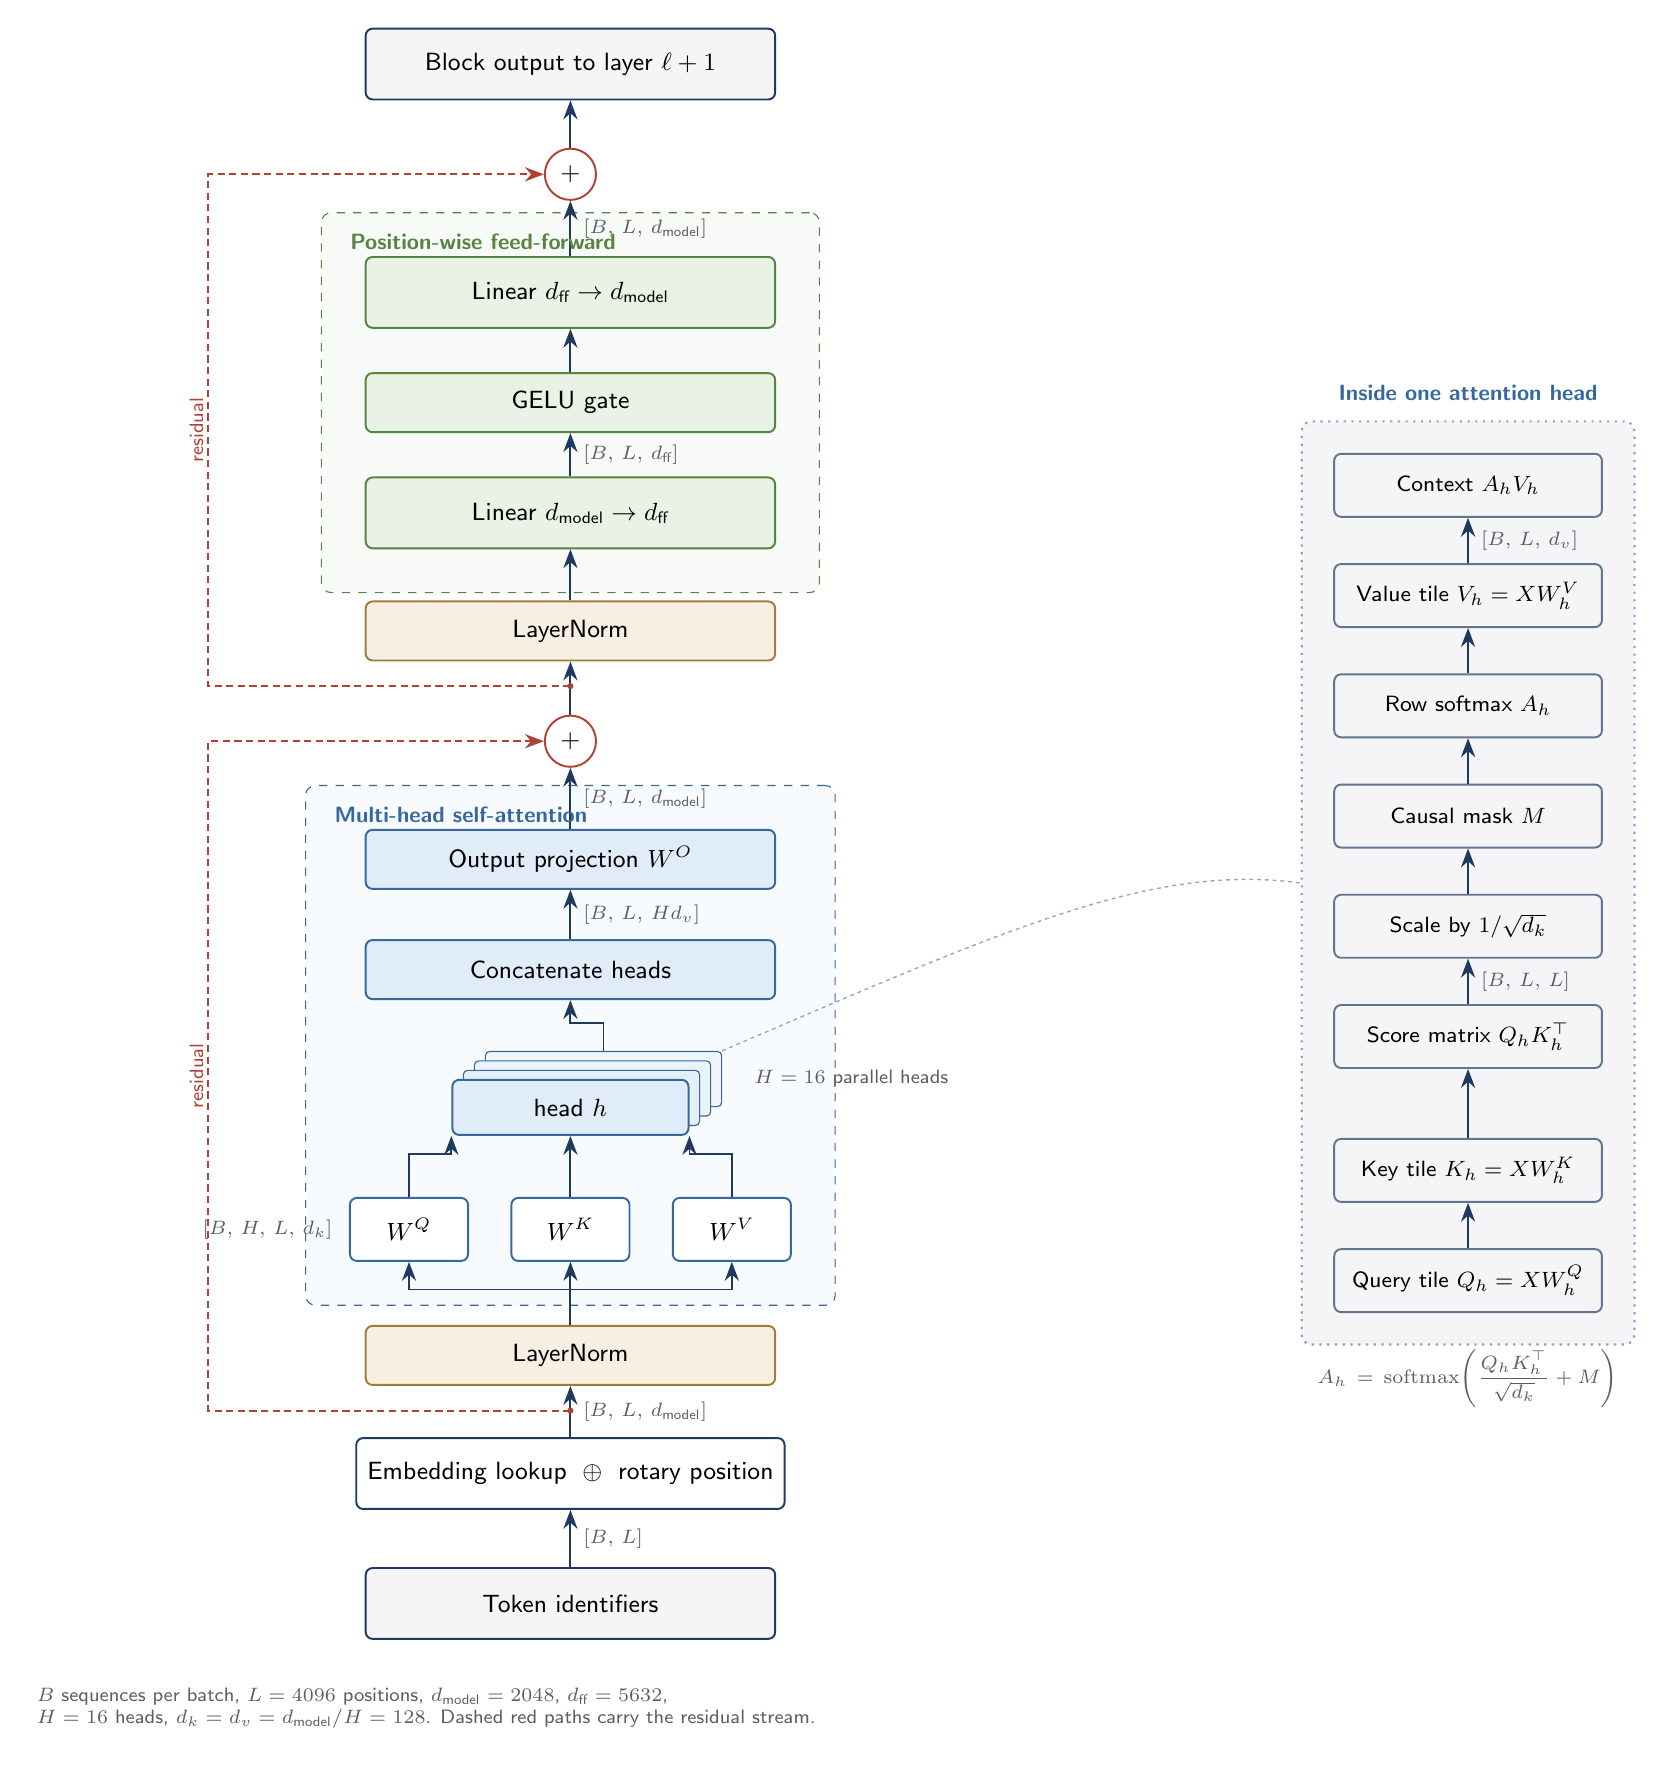
\begin{tikzpicture}[
    font=\sffamily,
    stage/.style={
      draw=shellink,line width=0.7pt,rounded corners=2.5pt,align=center,
      font=\sffamily\small,minimum width=52mm,minimum height=9mm,inner sep=4pt,
      fill=white},
    norm/.style={stage,draw=normline,fill=normfill,minimum height=7.5mm},
    attn/.style={stage,draw=attnline,fill=attnfill},
    ffn/.style={stage,draw=ffnline,fill=ffnfill},
    proj/.style={stage,draw=attnline,fill=white,minimum width=15mm,
      minimum height=8mm,font=\sffamily\small},
    small/.style={stage,minimum width=34mm,minimum height=8mm,
      font=\sffamily\footnotesize,fill=detailfill,draw=shellink!70},
    add/.style={circle,draw=residual,line width=0.7pt,fill=white,
      inner sep=0pt,minimum size=6.5mm,font=\small},
    flow/.style={-{Stealth[length=2.4mm,width=1.8mm]},line width=0.7pt,
      draw=shellink},
    res/.style={-{Stealth[length=2.4mm,width=1.8mm]},line width=0.7pt,
      draw=residual,dash pattern=on 2.6pt off 1.6pt},
    tie/.style={draw=shellink!45,line width=0.5pt,
      dash pattern=on 1.4pt off 1.4pt},
    tag/.style={font=\sffamily\scriptsize,text=shapetext,inner sep=1.5pt},
    head/.style={draw=attnline,fill=white,rounded corners=1.5pt,
      minimum width=30mm,minimum height=7mm,inner sep=0pt},
  ]

  \node[stage,fill=detailfill] (tokens) at (0,0)
    {Token identifiers};
  \node[stage] (embed) at (0,1.65)
    {Embedding lookup $\;\oplus\;$ rotary position};
  \node[norm] (ln1) at (0,3.15) {LayerNorm};

  \node[proj] (wq) at (-2.05,4.75) {$W^{Q}$};
  \node[proj] (wk) at (0,4.75) {$W^{K}$};
  \node[proj] (wv) at (2.05,4.75) {$W^{V}$};

  \node[head,fill=attnfill!45] (h4) at (0.42,6.66) {};
  \node[head,fill=attnfill!65] (h3) at (0.28,6.54) {};
  \node[head,fill=attnfill!85] (h2) at (0.14,6.42) {};
  \node[attn,minimum width=30mm,minimum height=7mm] (h1) at (0,6.30)
    {head $h$};
  \node[tag,anchor=west] at ($(h4.east)+(3.5mm,0)$)
    {$H = 16$ parallel heads};

  \node[attn,minimum height=7.5mm] (concat) at (0,8.05)
    {Concatenate heads};
  \node[attn,minimum height=7.5mm] (wo) at (0,9.45)
    {Output projection $W^{O}$};

  \node[add] (add1) at (0,10.95) {$+$};
  \node[norm] (ln2) at (0,12.35) {LayerNorm};

  \node[ffn] (up) at (0,13.85) {Linear $d_{\text{model}} \to d_{\text{ff}}$};
  \node[ffn,minimum height=7.5mm] (act) at (0,15.25)
    {GELU gate};
  \node[ffn] (down) at (0,16.65) {Linear $d_{\text{ff}} \to d_{\text{model}}$};

  \node[add] (add2) at (0,18.15) {$+$};
  \node[stage,fill=detailfill] (out) at (0,19.55)
    {Block output to layer $\ell + 1$};

  \draw[flow] (tokens) -- (embed)
    node[tag,midway,right=1mm] {\shape{[B,\,L]}};
  \draw[flow] (embed) -- (ln1)
    node[tag,midway,right=1mm] {\shape{[B,\,L,\,d_{\text{model}}]}};

  \draw[flow] (ln1.north) -- ++(0,0.45) -| (wq.south);
  \draw[flow] (ln1.north) -- ++(0,0.45) -| (wk.south);
  \draw[flow] (ln1.north) -- ++(0,0.45) -| (wv.south);

  \draw[flow] (wq.north) -- ++(0,0.55) -| (h1.south west);
  \draw[flow] (wk.north) -- ++(0,0.55) -| (h1.south);
  \draw[flow] (wv.north) -- ++(0,0.55) -| (h1.south east);

  \node[tag,anchor=east] at ($(wq.west)+(-1.5mm,0)$) {\shape{[B,\,H,\,L,\,d_{k}]}};

  \draw[flow] (h4.north) -- ++(0,0.35) -| (concat.south);
  \draw[flow] (concat) -- (wo)
    node[tag,midway,right=1mm] {\shape{[B,\,L,\,H d_{v}]}};
  \draw[flow] (wo) -- (add1)
    node[tag,midway,right=1mm] {\shape{[B,\,L,\,d_{\text{model}}]}};
  \draw[flow] (add1) -- (ln2);
  \draw[flow] (ln2) -- (up);
  \draw[flow] (up) -- (act)
    node[tag,midway,right=1mm] {\shape{[B,\,L,\,d_{\text{ff}}]}};
  \draw[flow] (act) -- (down);
  \draw[flow] (down) -- (add2)
    node[tag,midway,right=1mm] {\shape{[B,\,L,\,d_{\text{model}}]}};
  \draw[flow] (add2) -- (out);

  \coordinate (tap1) at (0,2.45);
  \coordinate (tap2) at (0,11.65);
  \draw[res] (tap1) -- ++(-4.6,0) |- (add1.west)
    node[tag,text=residual,pos=0.25,rotate=90,above] {residual};
  \draw[res] (tap2) -- ++(-4.6,0) |- (add2.west)
    node[tag,text=residual,pos=0.25,rotate=90,above] {residual};
  \fill[residual] (tap1) circle (1.1pt);
  \fill[residual] (tap2) circle (1.1pt);

  \begin{scope}[on background layer]
    \node[draw=attnline,dashed,rounded corners=3.5pt,inner sep=5.5mm,
          fill=attnfill!22,
          fit=(wq)(wv)(h4)(concat)(wo)] (attnbox) {};
    \node[draw=ffnline,dashed,rounded corners=3.5pt,inner sep=5.5mm,
          fill=ffnfill!35,
          fit=(up)(act)(down)] (ffnbox) {};
  \end{scope}
  \node[anchor=north west,font=\sffamily\footnotesize\bfseries,text=attnline]
    at ($(attnbox.north west)+(2.5mm,-1.6mm)$) {Multi-head self-attention};
  \node[anchor=north west,font=\sffamily\footnotesize\bfseries,text=ffnline]
    at ($(ffnbox.north west)+(2.5mm,-1.6mm)$) {Position-wise feed-forward};

  \node[small] (dq) at (11.4,4.10) {Query tile $Q_h = X W^{Q}_{h}$};
  \node[small] (dk) at (11.4,5.50) {Key tile $K_h = X W^{K}_{h}$};
  \node[small] (dmm) at (11.4,7.20) {Score matrix $Q_h K_h^{\top}$};
  \node[small] (dscale) at (11.4,8.60) {Scale by $1/\sqrt{d_k}$};
  \node[small] (dmask) at (11.4,10.00) {Causal mask $M$};
  \node[small] (dsm) at (11.4,11.40) {Row softmax $A_h$};
  \node[small] (dv) at (11.4,12.80) {Value tile $V_h = X W^{V}_{h}$};
  \node[small] (dctx) at (11.4,14.20) {Context $A_h V_h$};

  \draw[flow] (dq) -- (dk.south -| dq.north);
  \draw[flow] (dk) -- (dmm);
  \draw[flow] (dmm) -- (dscale)
    node[tag,midway,right=1mm] {\shape{[B,\,L,\,L]}};
  \draw[flow] (dscale) -- (dmask);
  \draw[flow] (dmask) -- (dsm);
  \draw[flow] (dsm) -- (dv);
  \draw[flow] (dv) -- (dctx)
    node[tag,midway,right=1mm] {\shape{[B,\,L,\,d_{v}]}};

  \node[anchor=south,font=\sffamily\footnotesize\bfseries,text=attnline]
    at (11.4,15.15) {Inside one attention head};
  \node[anchor=north,align=center,font=\sffamily\scriptsize,text=shapetext,
        text width=44mm]
    at (11.4,3.35)
    {$\displaystyle A_h = \operatorname{softmax}\!\left(
      \frac{Q_h K_h^{\top}}{\sqrt{d_k}} + M \right)$};

  \begin{scope}[on background layer]
    \node[draw=attnline!60,dotted,line width=0.8pt,rounded corners=3.5pt,
          inner sep=4mm,fill=detailfill,
          fit=(dq)(dctx)(dsm)] (detailbox) {};
  \end{scope}
  \draw[tie] (h4.north east) .. controls (5.6,8.6) and (7.4,9.4) ..
    (detailbox.west);

  \node[align=left,font=\sffamily\scriptsize,text=shapetext,anchor=north west]
    at (-6.9,-0.95)
    {$B$ sequences per batch, $L = 4096$ positions,
     $d_{\text{model}} = 2048$, $d_{\text{ff}} = 5632$,\\
     $H = 16$ heads, $d_k = d_v = d_{\text{model}}/H = 128$.
     Dashed red paths carry the residual stream.};

\end{tikzpicture}
\end{document}
